\documentclass[aspectratio=169,11pt]{beamer}

\usepackage[utf8]{inputenc}
\usepackage[T1]{fontenc}
\usepackage[spanish]{babel}
\usepackage{booktabs}
\usepackage{array}
\usepackage{graphicx}
\usepackage{xcolor}
\usepackage{amssymb}

\graphicspath{{Paper/figures/}{figures/}}

\definecolor{cjcblue}{HTML}{1F5EA8}
\definecolor{cjcyellow}{HTML}{F2C400}
\definecolor{cjcgray}{HTML}{4A4A4A}
\definecolor{cjclight}{HTML}{F5F6F7}

\setbeamertemplate{navigation symbols}{}
\setbeamercolor{normal text}{fg=black,bg=white}
\setbeamercolor{frametitle}{fg=cjcblue,bg=white}
\setbeamerfont{frametitle}{series=\bfseries,size=\large}
\setbeamerfont{title}{series=\bfseries,size=\Large}
\setbeamertemplate{itemize item}{\textcolor{cjcblue}{\scriptsize$\blacktriangleright$}}
\setbeamertemplate{itemize subitem}{\textcolor{cjcblue}{\tiny$\blacktriangleright$}}
\setlength{\parskip}{0.15cm}

\setbeamertemplate{footline}{
  \leavevmode
  \hbox{
    \begin{beamercolorbox}[wd=.74\paperwidth,ht=2.5ex,dp=1.1ex,leftskip=0.45cm]{author in head/foot}
      \scriptsize\color{cjcgray} CJC y Laboratorio de Economía de la Educación
    \end{beamercolorbox}
    \begin{beamercolorbox}[wd=.22\paperwidth,ht=2.5ex,dp=1.1ex,rightskip=0.45cm plus1fil]{date in head/foot}
      \scriptsize\color{cjcgray}\hfill \insertframenumber/\inserttotalframenumber
    \end{beamercolorbox}
  }
}

\newcommand{\fuente}[1]{\vspace{0.12cm}{\tiny\color{cjcgray}#1}}
\newcommand{\idea}[1]{{\large\textbf{\color{cjcblue}#1}}\par\vspace{0.18cm}}
\newcommand{\cjcbar}{\textcolor{cjcyellow}{\rule{0.18\textwidth}{1.5pt}}\hspace{0.3em}\textcolor{cjcblue}{\rule{0.72\textwidth}{1.5pt}}}

\title{Remuneración laboral por logro educativo en Colombia}
\subtitle{2010--2025}
\author{Centro Javeriano de Competitividad \\ Laboratorio de Economía de la Educación}
\date{Septiembre de 2026}

\begin{document}

\begin{frame}[plain]
\vspace{0.25cm}
\begin{columns}[c,totalwidth=\textwidth]
  \begin{column}{0.55\textwidth}
    
\includegraphics[height=1.15cm]{logo_cjc_palatino_horizontal.png}
  \end{column}
  \begin{column}{0.35\textwidth}
    \raggedleft
    
\includegraphics[height=1.25cm]{logo_lee.png}
  \end{column}
\end{columns}

\vspace{0.9cm}
{\color{cjcblue}\large Informes sobre la productividad en Colombia}

\vspace{0.18cm}
{\Huge\bfseries Remuneración laboral por logro educativo}

\vspace{0.15cm}
{\Large 2010--2025}

\vspace{0.35cm}
\cjcbar

\vfill
{\large Centro Javeriano de Competitividad}\\
{\large Laboratorio de Economía de la Educación}\\
{\normalsize Septiembre de 2026}
\end{frame}

\begin{frame}{Qué muestra el informe}
\idea{El informe compara dos formas de medir la remuneración laboral por logro educativo.}

\begin{itemize}
  \item La remuneración mensual por trabajador aproxima el ingreso laboral mensual equivalente de cada ocupado.
  \item La remuneración por hora trabajada compara cuánto se remunera una hora de trabajo.
  \item El periodo de análisis es 2010--2025 y excluye 2020 por el choque de la pandemia.
  \item Todas las cifras monetarias se expresan en pesos constantes de 2025.
\end{itemize}

\vspace{0.25cm}
La remuneración se interpreta como una aproximación a la productividad laboral. No es una medida directa de productividad, pero permite estudiar si el mercado remunera de manera distinta los logros educativos alcanzados por la población ocupada.

\fuente{Fuente: informe elaborado con microdatos de la GEIH del DANE.}
\end{frame}

\begin{frame}{La población ocupada alcanzó mayores logros educativos}
\idea{La composición del empleo cambió de forma marcada entre 2010 y 2025.}

\begin{center}
\scriptsize
\begin{tabular}{@{}lrrr@{}}
\toprule
Logro educativo & 2010 & 2025 & Dif. \\
\midrule
Sin educación o básica primaria & 48\% & 29\% & -19 p.p. \\
Básica secundaria & 6\% & 5\% & -2 p.p. \\
Educación media & 28\% & 37\% & +8 p.p. \\
Educación superior & 17\% & 30\% & +13 p.p. \\
\addlinespace
\textbf{Total ocupados} & \textbf{18,6 mill.} & \textbf{23,8 mill.} & \textbf{1,7\% anual} \\
\bottomrule
\end{tabular}
\end{center}

\vspace{0.25cm}
El cambio más importante no es solo que haya más ocupados. También hay una mayor proporción de trabajadores con educación media, formación técnica o tecnológica, pregrado universitario y posgrado.

\fuente{Fuente: cálculos propios con GEIH del DANE. Educación superior agrupa técnico o tecnológico, pregrado universitario y posgrado.}
\end{frame}

\begin{frame}{La remuneración aumenta con el logro educativo}
\idea{En 2025, quienes alcanzaron pregrado universitario ganaban cerca de cuatro veces lo que ganaban quienes no tenían ningún logro educativo.}

\begin{center}
\scriptsize
\begin{tabular}{@{}lrrr@{}}
\toprule
Logro educativo & Mensual & Hora & Razón mensual \\
\midrule
Ninguno & 0,9 & 5,0 & 1,0x \\
Básica primaria & 1,1 & 5,9 & 1,2x \\
Básica secundaria & 1,1 & 6,0 & 1,3x \\
Educación media & 1,5 & 7,5 & 1,6x \\
Técnico o tecnológico & 1,9 & 9,8 & 2,1x \\
Pregrado universitario & 3,5 & 18,9 & 4,0x \\
Posgrado & 6,9 & 37,6 & 7,8x \\
\bottomrule
\end{tabular}
\end{center}

\fuente{Fuente: cálculos propios con GEIH del DANE. Remuneración mensual en millones de pesos de 2025. Remuneración por hora en miles de pesos de 2025. La razón mensual compara cada logro con Ninguno.}
\end{frame}

\begin{frame}{El total creció más que cada logro educativo}
\idea{El promedio total aumentó porque cambió la composición educativa de la población ocupada.}

\begin{center}
\scriptsize
\begin{tabular}{@{}lrr@{}}
\toprule
Logro educativo & Mensual & Hora \\
\midrule
Ninguno & 0,7\% & 1,3\% \\
Básica primaria & 0,7\% & 1,3\% \\
Básica secundaria & 0,6\% & 1,0\% \\
Educación media & 0,4\% & 0,9\% \\
Técnico o tecnológico & -0,1\% & 0,3\% \\
Pregrado universitario & -0,6\% & -0,4\% \\
Posgrado & 0,0\% & 0,0\% \\
\midrule
\textbf{Total} & \textbf{1,6\%} & \textbf{2,0\%} \\
\bottomrule
\end{tabular}
\end{center}

\vspace{0.18cm}
El crecimiento del total fue mayor que el crecimiento observado dentro de casi todos los logros educativos. Esa diferencia anticipa el resultado de la descomposición.

\fuente{Fuente: cálculos propios con GEIH del DANE. Tasas anuales para 2010--2025.}
\end{frame}

\begin{frame}{Descomposición de la remuneración promedio}
\idea{El mayor logro educativo de la población ocupada explica la mayor parte del aumento agregado.}

\begin{center}
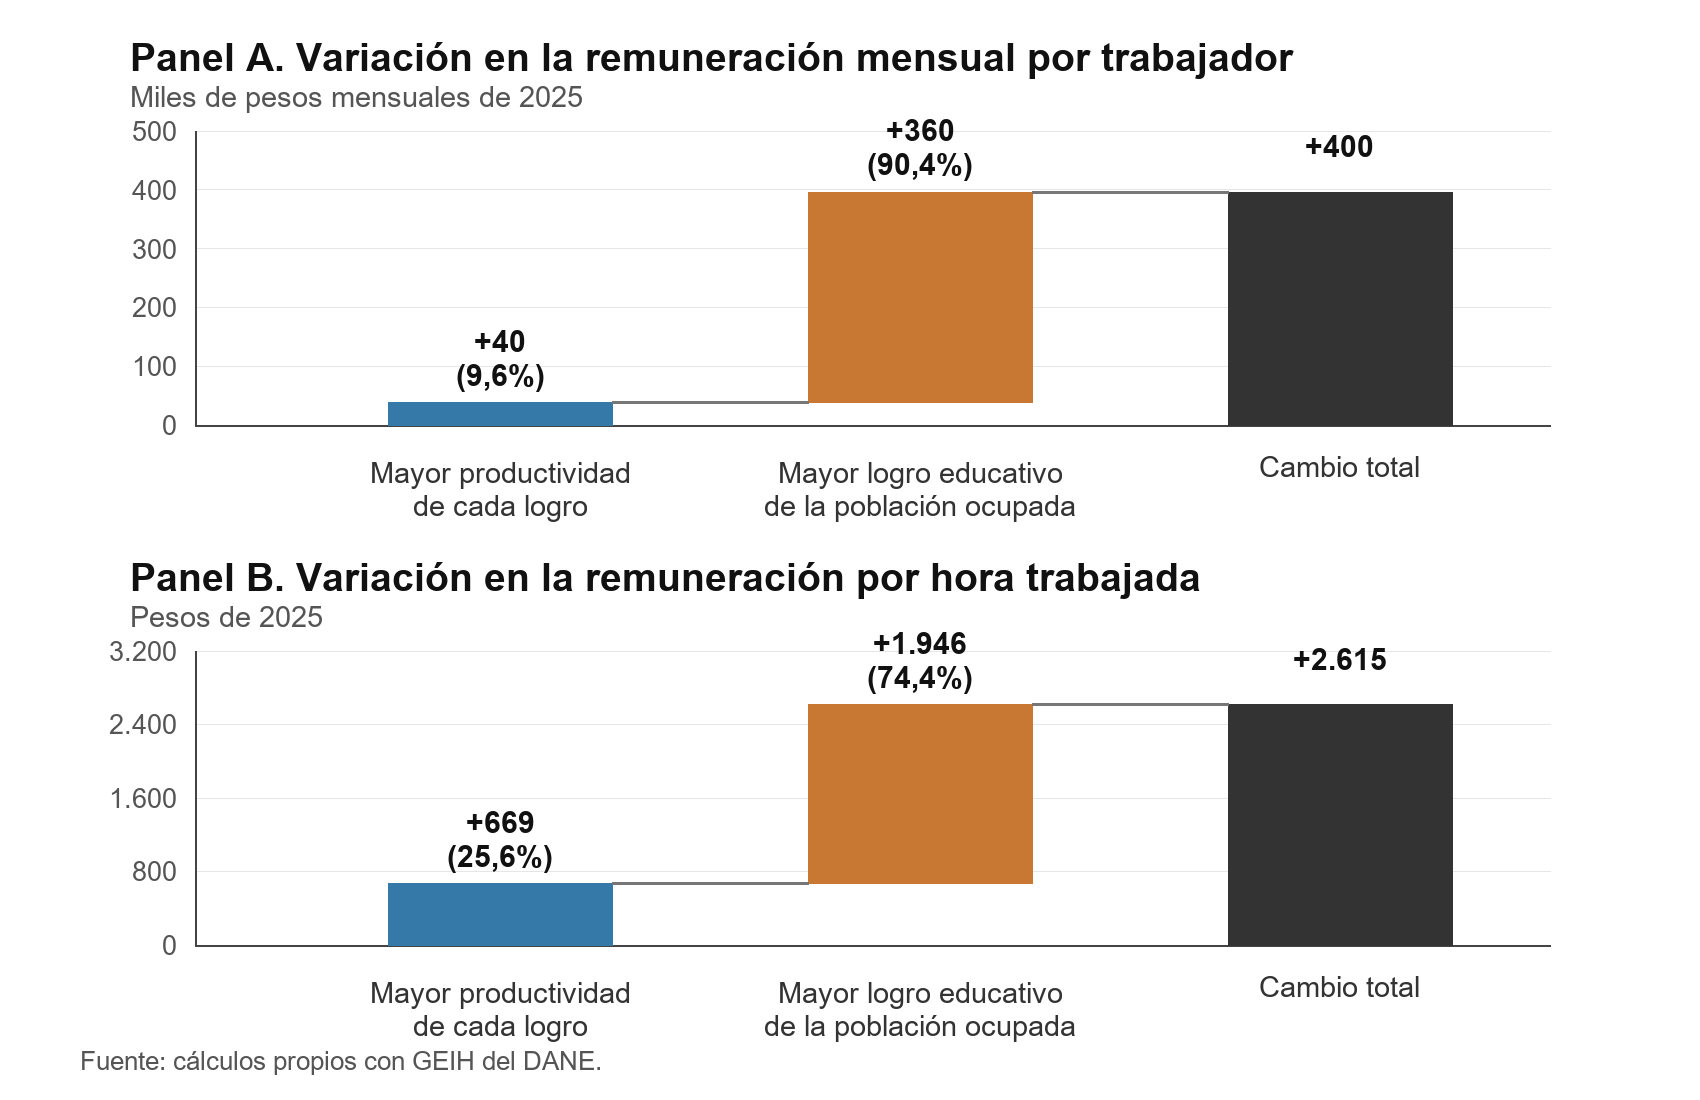
\includegraphics[width=0.95\textwidth,height=0.59\textheight,keepaspectratio]{fig_descomposicion_remuneracion_educacion_cascada.png}
\end{center}

\fuente{Fuente: cálculos propios con GEIH del DANE.}
\end{frame}

\begin{frame}{Pregrado universitario}
\idea{El pregrado universitario sigue estando mejor remunerado, pero su remuneración promedio real fue menor que en 2010.}

\begin{center}
\scriptsize
\begin{tabular}{@{}lrr@{}}
\toprule
Indicador & 2010 & 2025 \\
\midrule
Remuneración mensual promedio & 3,8 & 3,5 \\
Remuneración por hora promedio & 20,2 & 18,9 \\
Razón mensual frente a Ninguno & 4,8x & 4,0x \\
Razón por hora frente a Ninguno & 4,9x & 3,8x \\
Ocupados & 1,3 mill. & 2,8 mill. \\
\bottomrule
\end{tabular}
\end{center}

\vspace{0.2cm}
El resultado no implica que estudiar pregrado haya dejado de pagar. Implica que, en promedio, la remuneración real de este logro no creció durante el periodo estudiado.

\fuente{Fuente: cálculos propios con GEIH del DANE. Remuneración mensual en millones de pesos de 2025. Remuneración por hora en miles de pesos de 2025.}
\end{frame}

\begin{frame}{Jóvenes con pregrado universitario}
\idea{Entre ocupados de 25 a 29 años con pregrado universitario, la remuneración promedio también cayó.}

\begin{center}
\scriptsize
\begin{tabular}{@{}lrr@{}}
\toprule
Indicador & 2010 & 2025 \\
\midrule
Ocupados & 228 mil & 494 mil \\
Promedio mensual & 3,3 & 3,0 \\
Mediana mensual & 2,5 & 2,5 \\
Cerca del salario mínimo & 6\% & 13\% \\
Promedio por hora & 17,6 & 16,3 \\
\bottomrule
\end{tabular}
\end{center}

\vspace{0.2cm}
La GEIH no identifica el año de graduación. Por eso este grupo aproxima a los recién egresados, pero no los observa directamente.

\fuente{Fuente: cálculos propios con GEIH del DANE. Remuneración mensual en millones de pesos de 2025. Remuneración por hora en miles de pesos de 2025.}
\end{frame}

\begin{frame}{Distribución de jóvenes con pregrado universitario}
\idea{La distribución permite ver si el promedio oculta cambios en la dispersión.}

\begin{center}
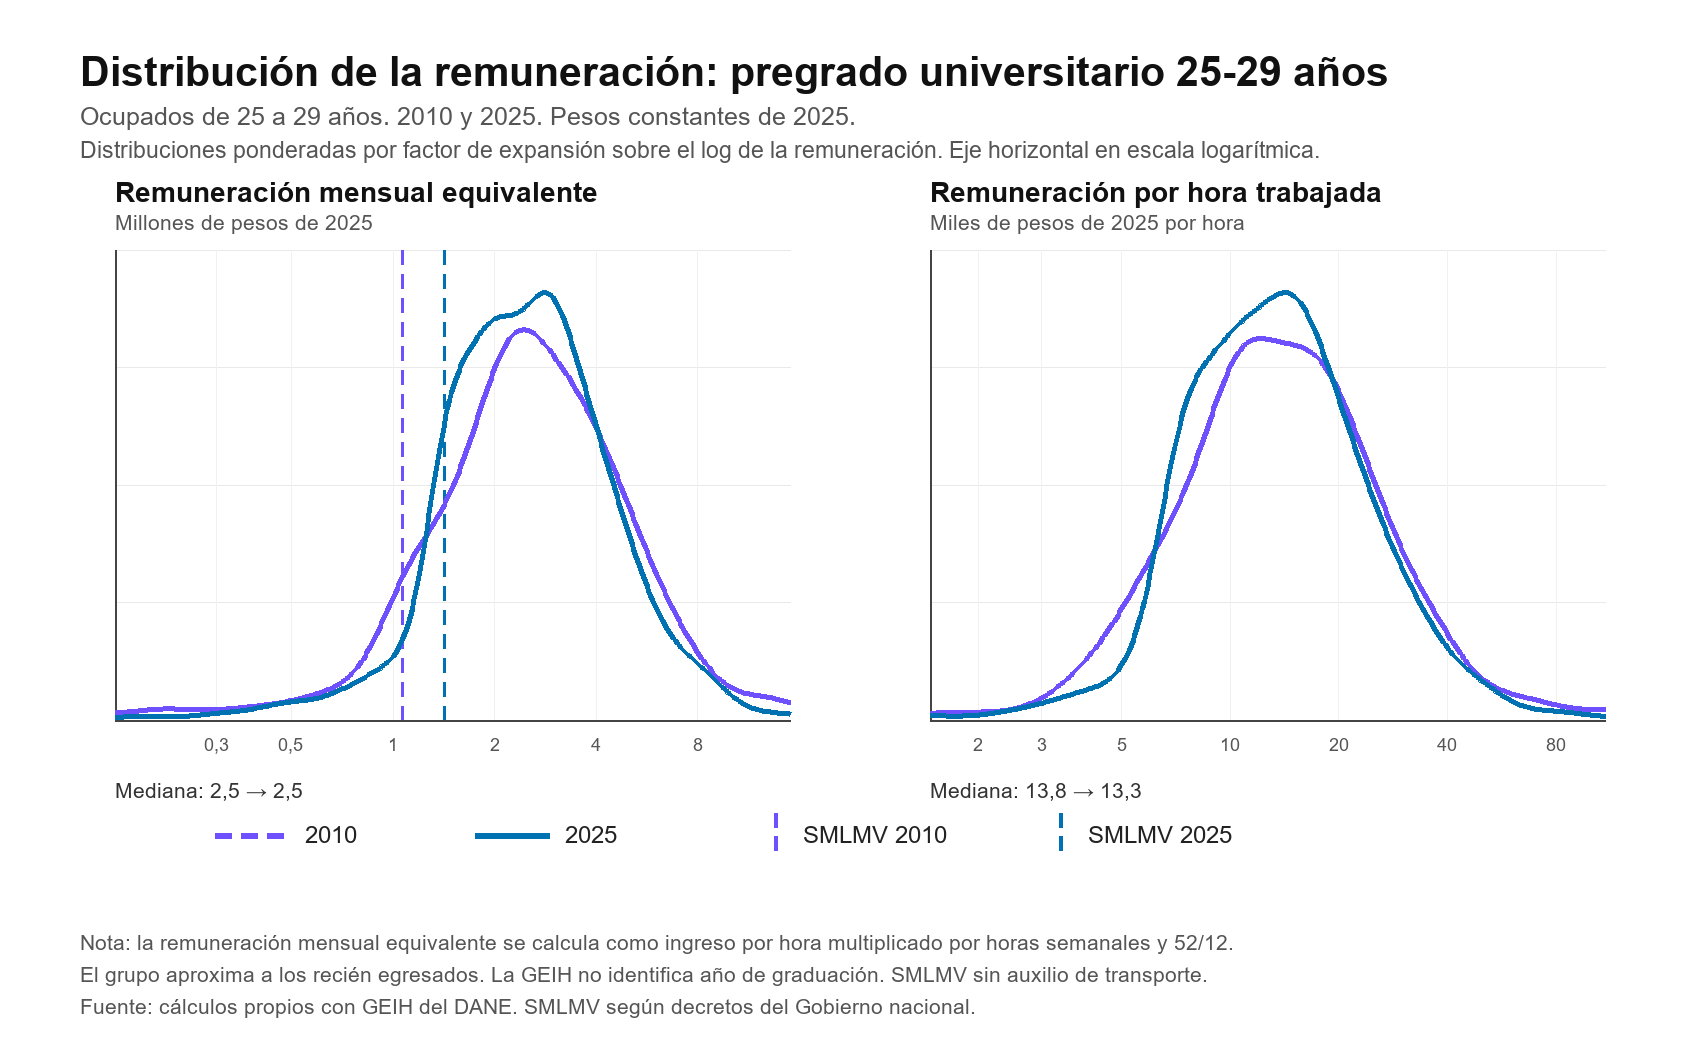
\includegraphics[width=0.95\textwidth,height=0.59\textheight,keepaspectratio]{fig_kernel_pregrado_universitario_25_29_2010_2025.png}
\end{center}

\fuente{Fuente: cálculos propios con GEIH del DANE.}
\end{frame}

\begin{frame}{Educación superior desde 2021}
\idea{La apertura de la pregunta muestra diferencias dentro de quienes alcanzaron educación superior.}

\begin{center}
\scriptsize
\begin{tabular}{@{}lrrr@{}}
\toprule
Logro educativo & 2021 & 2025 & Crec. anual \\
\midrule
Técnica profesional & 1,6 & 1,7 & 1,8\% \\
Tecnológica & 1,9 & 2,1 & 1,9\% \\
Pregrado universitario & 3,3 & 3,1 & -1,3\% \\
Especialización & 6,7 & 6,1 & -2,3\% \\
Maestría & 7,3 & 7,5 & 0,4\% \\
Doctorado & 8,7 & 9,3 & 1,6\% \\
\bottomrule
\end{tabular}
\end{center}

\vspace{0.2cm}
La remuneración aumentó en formación técnica profesional, tecnológica, maestría y doctorado. En cambio, cayó para pregrado universitario y especialización.

\fuente{Fuente: cálculos propios con GEIH del DANE. Remuneración mensual en millones de pesos de 2025.}
\end{frame}

\begin{frame}{Trayectoria anual}
\idea{Las series anuales muestran el contraste entre el total y cada logro educativo.}

\begin{center}
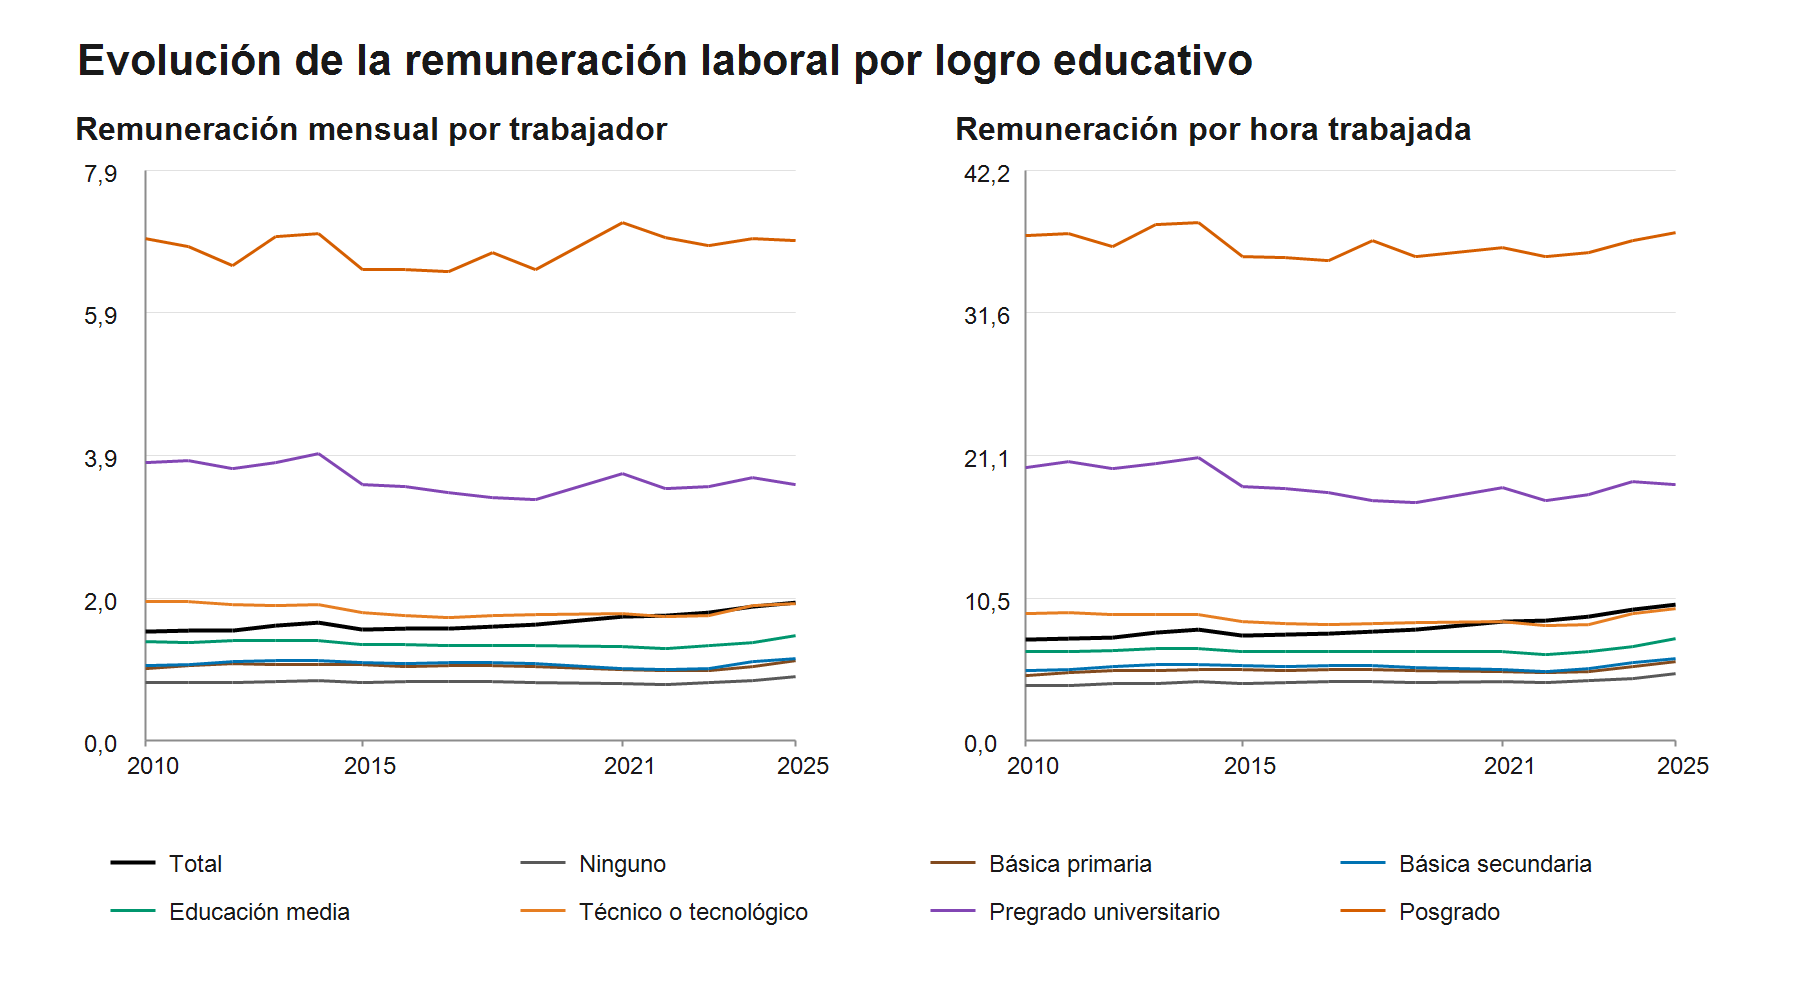
\includegraphics[width=0.95\textwidth,height=0.60\textheight,keepaspectratio]{fig_remuneracion_educacion_series_comparables.png}
\end{center}

\fuente{Fuente: cálculos propios con GEIH del DANE. La serie excluye 2020.}
\end{frame}

\begin{frame}{Conclusiones}
\idea{El mayor logro educativo elevó la remuneración promedio, pero no resolvió el bajo crecimiento dentro de cada logro.}

\begin{itemize}
  \item La población ocupada alcanzó mayores logros educativos entre 2010 y 2025.
  \item Esa recomposición explica la mayor parte del aumento agregado de la remuneración laboral.
  \item La remuneración real dentro de varios logros educativos creció poco o cayó.
  \item El caso de pregrado universitario merece seguimiento, especialmente entre trabajadores jóvenes.
  \item La agenda del país debe sostener el aumento del logro educativo y lograr que ese mayor logro se traduzca en mayor productividad y mejor remuneración.
\end{itemize}

\end{frame}

\end{document}
